\documentclass{article}
\usepackage{pgf,tikz,tikzscale} 
\usepackage{amssymb}
\usepackage{tcolorbox}
\usepackage{xcolor}
\usepackage[utf8]{inputenc}
\usepackage[english]{babel}
\usepackage{multicol}
\usepackage{enumerate}	
\usepackage{graphicx,lipsum,pgfplots} 
\usepackage{amsmath, amsthm}                 
\usepackage[top=1in,bottom=1in, left=.5in, right=.5in] {geometry}  
\usepackage{fancyhdr}       



\pagestyle{fancy}              
\lhead{Math 5910 \newline Exam 1}   
\rhead{Warren Keil}







\begin{document}
\setlength{\parindent}{0cm}   %%%%%%%% KEEP THIS  for block style para. 



%%%%%%%%%%%%%%%%%        1a   %%%%%%%%%%%%%%%%%%%%
\textbf{1a.}  Write a PDE model for the following scenario. An irrigation ditch of length \(L\) is used to water crops on a farm. The initial pesticide concentration in the ditch in 5\(\mu M\). No new pesticide will be added to ditch. Water does not flow in this ditch. The pesticide does diffuse through the water with diffusion coefficient \(D\). The ditch is capped on left end and has a 100\% effective filter on the right end. 


\vspace{3mm}
\textit{Solution.}  Since the dimension of the ditch is given as simply length, we know this PDE will have one spatial dimension, \(x\). We also will have a time variable \(t\) as implied in the problem. Since we are given that water does not flow, then we know that we will not have advection in our model. We do know that this will be a diffusion model as stated with diffusion coefficient \(D\). We also know that our flux \( \phi = 0\) for when \( x \leq 0\). And since this is a diffusion only problem, our flux is \( \phi = -Du_x \). Since the farmer is not adding pesticide, and we are not concerned about the concentration outside the region, then our model is justified in not having a source or sink term. We also note that since our initial condition was given in \(\mu\!M\), then all of the \(A\) terms listed next will denote micro-moles, and all of the \(L\) terms will denote the unit of length the corresponds to one liter of water in the ditch. \(( \star) \)

\begin{align*} 
u &= \text{concentration of pesticide at \(x\) at time \(t\);  units: \(\frac{\text{A}}{\text{L}}\) }. \\
u_t &=  \text{ rate of change of u over time; units = } \frac{A}{TL}\\
\phi&= -Du_x(x,t) = \text{flux of pesticide at \(x\) at time \(t\);  units of D: \(\frac{L^2}{T}\); units of \(u_x= \frac{A}{L^2} \). }\\
\phi_x &= -Du_{xx} = \text{rate of change of flux; units= } \frac{ L^2 A}{T L^3} =  \frac{  A}{T L} 
\end{align*}

And so our PDE is:  

\begin{align*}
&& u_t - Du_{xx} &= 0 ,\hspace{2mm} D>0,  \hspace{2mm}0<x<l,\hspace{2mm}  t>0 	 	&     &     \\
s.t. & &         u(x,0) &=   5 \mu M,      \hspace{2mm}0<x<l,\hspace{2mm}  t=0          &      \text{Initial condition}    &         \\
\hspace{40mm}  & &      Du_{x}(0,t)  &= 0               &      \text{B.C., ditch is capped at left end}     & \\
 & &  u(l,t) &= 0  & \text{B.C., the filter removes all pesticide at }l
 \end{align*}


%%%%%%%%%%%%%%%%%        1b   %%%%%%%%%%%%%%%%%%%%
\vspace{3mm}
\textbf{1b.} Write a PDE model for the following scenario. There is another irrigation ditch that starts off with out any pesticide in it. There are now filters at both ends of the ditch and water flows from left to right at advection speed \(c\). Pesticide now seeps into the ditch continuously and uniformly at a constant rate \(r\). Note: \(r\) has dimensions \(\frac{\mu M}{\text{time}}\). 

\vspace{3mm}
\textit{Solution.}  Now, our model becomes an advection-diffusion model with a source term. The model is still diffusive in nature since its the same pesticide dissolved in water. The model is advective as given in the problem. And the model has a source term now since the problem states that the pesticide leeches in to the ditch. Since nothing has change in terms of the diffusive component of flux, it will remain the same \(-Du_{x}\). The fact that the problem states that the water moves at speed \(c\) means the advection part of our model is \(cu\).  Since there are filters on both ends of the ditch, we simply only consider the length of the ditch for \( x \in (0,l)\). Since the problem states that ditch started off pesticide free, then we know the initial condition is \( u(x,0) = 0 \mu\! M,  \forall x \). And lastly, the source term becomes \( f(x,t) = r , \forall x, \forall t>0 \). Writing this formally, we get, 
\begin{align*}
&& u_t -Du_{xx} +cu_x&= r, \hspace{2mm} 0<x<l, \hspace{2mm} 0 \leq t, \hspace{2mm}0< D,c,r&     &     \\
 s.t.& &       u(x,0) &= 0, \hspace{2mm}0<x<l, \hspace{2mm} t=0     &    \text{Initial Condition} &         \\
 & &        u(0,t)&=0, \hspace{2mm} 0\leq t           &\text{B.C., filter remove pesticide at }x=0            &         \\
 & &        u(l,t)&=0, \hspace{2mm} 0\leq t                 &   \text{B.C., filter remove pesticide at }x=l         &               
\end{align*}





%%%%%%%%%%%%%%%%%        2a    %%%%%%%%%%%%%%%%%%%%
\newpage
\textbf{2a.} Consider the two concentric spheres of radii \( \rho=.5\) and \( \rho=4\). The inner sphere is held at \(20^{\circ}\) and the outer sphere satisfies the condition \(u_\rho (4,\theta, \phi)=1\). Write the differential equation and boundary conditions needed to find the steady state temperature in the region between the two spheres. 

\vspace{3mm}
\textit{Solution.} Since the boundary condition that were given do not change or depend the angles \(\theta \) or \( \phi\), then we can assume that the temperature between the two spheres is constant and unchanging with respect to \(\theta \) or \(\phi\). Thus, our model will only depend on the variable \(\rho\). Using Laplace's Equation in spherical coordinates, we get, 
\begin{align*}
&& u''(\rho) + \frac{2}{\rho} u'(\rho) &= 0,  \hspace{2mm} .5<\rho<4,  &     & \\
s.t. &&  u(.4) &= 20    &  \text{ B.C. of \(u\) }& \\
&&  u'(4) &= 1  &  \text{B.C. of \(u'\) }&
\end{align*}

%%%%%%%%%%%%%%%%%        2b    %%%%%%%%%%%%%%%%%%%%
\vspace{3mm}
\textbf{2b.} Find the steady state temperature. 

\vspace{3mm}
\textit{Solution.}  To find the steady state temperature, will solve the ODE that our model has  been reduced to.

\begin{align*}
 &&     u''(\rho) + \frac{2}{\rho} u'(\rho) &= 0     &     &   \\
 &    &   \rho^2u'' + 2\rho u'  &=0      &     \text{  }&   \\
 &&   \frac{d}{d\rho}(\rho^2u') &=0      &      \text{}&   \\
 &&    \int \frac{d}{d\rho}(\rho^2u') d\rho &= \int 0 d\rho     &      \text{  }&   \\
 &&    \rho^2 u'  &=   c_1   &      \text{  }&   \\
 &&   u' &=  \frac{c_1}{\rho^2}  &  \clubsuit & \\
 &&    \int u' d \rho  &=  \int c_1 \rho^{-2} d\rho   &     \text{  } &   \\
 &&     u &= c_2 \rho^{-1} + c_3.     &     \text{ where }c_2=-c_1&  
\end{align*}
Now that we have the general form the equation, we use the boundary conditions to solve to the constants. 
\begin{align*}
\text{we refer to } \clubsuit && \text{   } u'(4)= \frac{c_1}{16}&=1     & u(.5) = \frac{-16}{.5} + c_3 &=20      \\
&&  c_1 &= 16 &            -32+c_3 &=  20  \\
&&  c_2 &= -16  &   c_3 &= 52
\end{align*}
Therefore we have our equation,
\[  u = \frac{-16}{\rho} + 52.   
\]
And we verify this with mathematica:
\begin{verbatim}
f[r_] := -16/r + 52 
D[f[r], {r, 2}] + (2/r)*D[f[r], {r, 1}]=0
\end{verbatim}

\begin{flushright}
\qed
\end{flushright}
%%%%%%%%%%%%%%%%%        3a i    %%%%%%%%%%%%%%%%%%%%
\newpage
\textbf{3a. (i)} For the solution surfaces plotted below, say what type of PDE \(u\) solves. Justify your answer. 

\vspace{0mm}



\begin{multicols}{2}
\textit{Solution.} The first picture is a picture of a solution to a diffusion PDE. We know this because the rate of change with respect to \(x\) is symmetrical about some value of \(x\); in this case, it looks like it's symmetrical about \(x=0\). This fact paired with the observation that the model is getting smaller everywhere as time increases tells us that this is a diffusion model. Furthermore, if we imagine taking cross sections of this model for fixed \(t\) values, we will find that \(u\) appears to have a normal curve a smaller peak as time gets larger.  Finally, the plot created on the right was constructed using a diffusion only PDE model. It looks very similar to the model presented on the exam. 

\begin{flushright}
\includegraphics[scale=.55]{3ddiffuse}
\end{flushright}
\end{multicols}


  

%%%%%%%%%%%%%%%%%        3a ii    %%%%%%%%%%%%%%%%%%%%
\vspace{3mm}
\textbf{3a. (ii)} For the solution surfaces plotted below, say what type of PDE \(u\) solves. Justify your answer. 

\begin{multicols}{2}
\textit{Solution.} \begin{flushleft}
\includegraphics[scale=.55]{3dadvecdiff}
\end{flushleft}

This surface is a solution to an advection-diffusion PDE model. We know it is advective because there is a defined peak at some line \(x=ct\) for some \( c\in \mathbb{R}\). We know it is diffusive because is we find what the value of \(c\), then we can easily transform our model back to a diffusion model by a change of variable. Then everything mentioned in part (i) would be more apparent here. That is, the model is diffusing over time, or getting smaller everywhere with respect to \(t\). Finally, the plot on the left was created using an advection diffusion model in Mathematica\( \textregistered\) and it looks extremely similar to the model posted in the exam.  
\end{multicols}



%%%%%%%%%%%%%%%%%        3a iii    %%%%%%%%%%%%%%%%%%%%
\vspace{3mm}
\textbf{3a. (iii)} For the solution surfaces plotted below, say what type of PDE \(u\) solves. Justify your answer. 

\begin{multicols}{2}
\textit{Solution.} This surface is a solution to an advection PDE. We know this because the value of \(u\) is moving along the line \(x=ct\) and some constant speed \(c\). We know it is not a solution to a wave equation because we only have one ridge along the surface. And finally, the plot of the right was created using a solution to an advection only PDE model and it looks very similar to the plot on the exam. 

\begin{flushright}
\includegraphics[scale=.55]{3dadvec}
\end{flushright}
\end{multicols}


%%%%%%%%%%%%%%%%%        3b    %%%%%%%%%%%%%%%%%%%%
\vspace{3mm}
\textbf{3b.}  Plot time snapshots of 
\[
u(x,t) = \frac{1}{2} \left(e^{-(x-2t)^2} + e^{-(x+2t)^2} \right) + \frac{1}{4} \left( \sin(x+2t) - \sin(x-2t)) \right).
\]
Describe what happens to \(u\) as time goes on. 


\vspace{3mm}
\textit{Solution.} We notice that as time gets sufficiently large, then the term \( e^{-(x-2t)^2} + e^{-(x+2t)^2}\) will get arbitrarily close to zero and we can disregard it. Thus, the steady state model will become: 
\[
u(x,t) = \frac{1}{4} \left( \sin(x+2t) - \sin(x-2t) \right).
\]
We see that this model oscillates like a normal sine curve in the \(x\) direction and it acts like \(\sin(2t)\) (stretched out) in the \(t\) direction. 
\vspace{15mm}

\begin{centering}
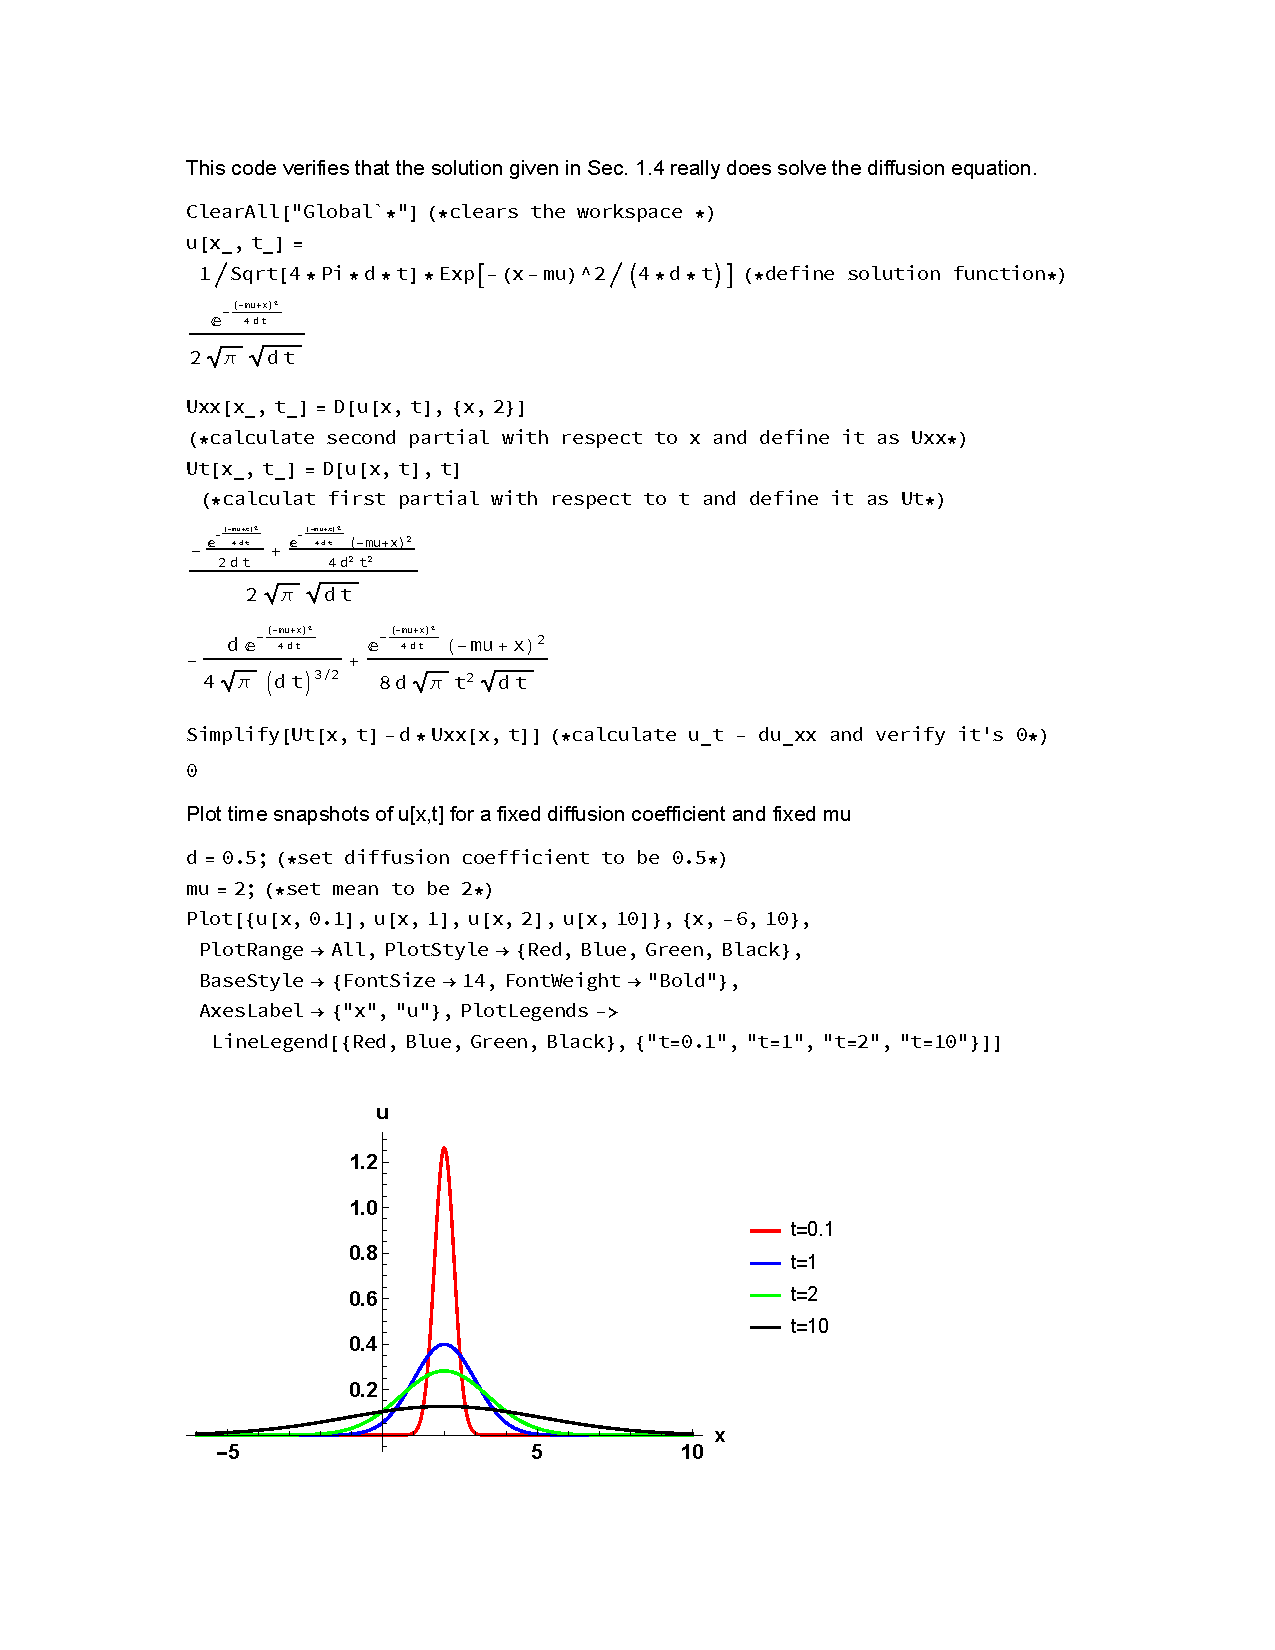
\includegraphics[scale=1.35]{timesnap}
\end{centering}

\begin{tcolorbox}

\textbf{Legend}
\begin{align*}
 \color{red} t=.5  &&  \color{blue} t=2 && \color{green} t=5  &&  t=7
\end{align*}

\end{tcolorbox}

\newpage
\textbf{4a.} Consider the wave equation 
\begin{align}
u_{tt} &= c^2u_{xx},   \hspace{8mm} 0<x<l, \hspace{5mm} t>0  \\
u_x(0,t) &= u_x(l,t) = 0,  \hspace{8mm} t\geq0  \\
u(x,0) &=f(x),  \hspace{8mm} u_t(x,0)=g(x), \hspace{8mm} 0 \leq x\leq l
\end{align}
with \(c>0\) constant. The total energy of the string is given by the equation 
\[
E(t) = \frac{1}{2} \int_{0}^l (u_t^2+c^2u_x^2 )dx. 
\]
Show that the energy is conserved. 

\vspace{3mm} 
\textit{Solution.} Let \(E(t) = \frac{1}{2} \int_{0}^l (u_t^2+c^2u_x^2 )dx\). To show that energy is conserved, we need to show that the energy of the system describe by the function \(E(t)\) does not change with respect to time. That is, we need to show that \(\frac{d}{dt} E(t)=0 \). We also observe that if we multiply both sides of the wave equation by \(u_t\), we get \(u_tu_{tt} = c^2u_tu_{xx}\). Notice: 
\begin{align*}
&& E'(t) &=  \frac{d}{dt} \left[ \frac{1}{2} \int_{0}^l (u_t^2+c^2u_x^2 )dx \right]   &   & \\
&& &=  \frac{1}{2} \int_{0}^l \left(\frac{d}{dt}u_t^2+\frac{d}{dt}c^2u_x^2 \right)dx  &   &\\
&& &= \frac{1}{2} \int_{0}^l \left( 2u_tu_{tt}+ 2c^2u_xu_{xt} \right) dx  &  \text{by using chain rule of derivatives} & \\
&& &= \frac{1}{2} \int_{0}^l \left( 2c^2u_tu_{xx}+ 2c^2u_xu_{xt} \right) dx  &  u_{tt} = c^2u_{xx} \Rightarrow u_tu_{tt} = c^2u_tu_{xx}& \\
 \hspace{50mm} && &= \frac{2c^2}{2}\left[ \int_{0}^l u_tu_{xx} dx +\int_{0}^l u_xu_{xt}  dx \right] & \text{since we have same limits of integration}&\\
&& &= c^2 \left[\left[u_tu_x \right]_0^l -\int_{0}^l u_xu_{xt} dx +\int_{0}^l u_xu_{xt}  dx \right] &  \text{by integration by parts }& \\
&& &= c^2 \left[\left[0- 0 \right] -\int_{0}^l u_xu_{xt} dx +\int_{0}^l u_xu_{xt}  dx \right] &  \text{B.C.  }u_x(0,t) = u_x(l,t) = 0 & \\
&& &= c^2 \left[\int_{0}^l u_xu_{xt} dx -\int_{0}^l u_xu_{xt}  dx \right] &  &  \\
&& &= 0  &  &  
\end{align*}
Thus, we have shown the energy of this system does not change with respect to time, and energy is conserved. 

\begin{flushright}
\( \qed \)
\end{flushright}

\newpage
\textbf{4b.} Assume \(u(x,t) \) and \(v(x,t)\) are both solutions to Equations \((1)-(3)\). Let \(w(x,t)=u(x,t)-v(x,t)\). Show that \(w\) satisfies Equation \((1)\), and find the new boundary and initial conditions for \(w\). 


\vspace{3mm} 
\textit{Solution.} As suggested, we let \(w(x,t)=u(x,t)-v(x,t)\) where \(u\) and \(v\) satisfy Equations \((1)-(3)\). To show that \( w\) satisfies equation \((1)\), we take the following derivatives:
\begin{align}
w_t &= u_t - v_t \\
w_{tt} &=u_{tt}-v_{tt} \\
w_x &= u_x + v_x \\
w_{xx} &= u_{xx} + v_{xxz} \\ 
c^2w_{xx} &= c^2u_{xx} - c^2v_{xx}
\end{align} 
Now we use the fact that since \(u \) and \(v\) satisfy Equation 1, then \(u_{tt}=c^2u_{xx}\) and \(v_{tt}=c^2v_{xx} \). Thus, we have 
\[
w_{tt} = u_{tt}-v_{tt} = c^2u_{xx}-c^2v_{xx} = c^2(u_{xx}-v_{xx} )= c^2w_{xx}.
\] 
\begin{flushright}
\( \qed \)
\end{flushright}

The new boundary and initial conditions for \(w\) are given directly from equations (2)-(7).

\begin{align}
w_x(0,t) &= u_x(0,t)-v_x(0,t) = 0 -0 = 0, \\
w_x(l,t) &= u_x(l,t)-v_x(l,t) = 0 -0 = 0, \\
w(x,0) &= u(x,0) - v(x,0)    = f(x) - f(x) =0,  \\
w_t(x,0) &= u_t(x,0) - v_t(x,0)  = g(x) - g(x) =0. 
\end{align}








\newpage
\textbf{4c.} Using part \((a)\), and paying attention to the quantity \(E(0)\), show that \(w(x,t)=0\), and thus, the wave equation's solution is unique. 

\vspace{3mm} 
\textit{Solution.} Let \(E(t) \) now describe the energy equation as applied to \(w\), \(E(t)=\frac{1}{2} \int_0^l w_t^2 + c^2w_x^2 dx\). We first will observe \(E(0)\). Notice, 

\begin{align*}
  & & E(0)&=\frac{1}{2} \int_0^l w_t(x,0)^2 + c^2w_x(x,0)^2 dx     &   &    \\
  & &     &=\frac{1}{2} \int_0^l 0+ c^2w_x(x,0)^2 dx       &\text{from Equation (12)} &    \\
  & &     &=   \frac{c^2}{2} \int_0^l w_x(x,0)^2 dx    &   &   
  \end{align*}
  
  We now argue why the quantity \( \frac{c^2}{2} \int_0^l w_x(x,0)^2 dx \) is equal to zero. We already showed in Equation (11) that \(w(x,0) = 0,   \forall x\) when \(t=0\). Thus, it is not changing with respect to \(x\) when \(t=0\). Therefore, \(w_x(x,0) = 0\). Hence, 
  \[ 
  E(0) =   \frac{c^2}{2} \int_0^l w_x(x,0)^2 dx =  \frac{c^2}{2} \int_0^l 0 dx = 0 .
  \]
Thus, since \(E(0) = 0 \), and \(E'(t)= 0\) then it follows that \(E(t)\) is zero for all \(t\). We now can make the following argument using iff strings: 
\begin{align*}
  & & E(t) = 0&=\frac{1}{2} \int_0^l w_t^2 + c^2w_x^2 dx     &   &     \\
  &\iff	&	0&=\int_0^l w_t^2 + c^2w_x^2 dx	&	&  	\\
\hspace{38mm}  &\iff	 	&	0&=\int_0^l w_t^2 dx+ \int_0^lc^2w_x^2 dx & \text{we can remove \(c^2\) since it is constant} &  	\\
  &\iff		&	0&=\int_0^l w_t^2 dx,	 \hspace{10mm}	0=\int_0^lw_x^2 dx  &\text{since both are nonnegative} &	\\
  &\iff	&	w_t&=0, 	\hspace{10mm} w_x=0. & \text{since definite integrals equals zero in both cases}&  	 
  \end{align*}

Now, we know from Equation (11) that the initial value for \(w\) is zero for all \(x\). We then showed the the derivatives of \(w\) in both the \(x\) and \(t\) directions were zero for all \(x\) and \(t\). Therefore,\( w(x,t) = 0, \forall x,t \). This means that \(w\) starts at equally zero and does not change in either of the two directions. Thus \( u=v,  \forall x,t\) and our solution is unique. 


\begin{flushright}
\( \blacksquare \)
\end{flushright}








\end{document}